%%
% TUM Corporate Design LaTeX Templates
% Based on the templates from https://www.tum.de/cd
%
% Feel free to join development on
% https://gitlab.lrz.de/tum-templates/templates
% and/or to create an issue in case of trouble.
%
% tum-article class for scientific articles, reports, exercise sheets, ...
%
%%

\documentclass[twocolumn]{tum-article}
%\documentclass[twocolumn, german]{tum-article}
%\documentclass[times, twocolumn]{tum-article}
%\documentclass[times]{tum-article}
%\documentclass{tum-article}

\usepackage{lipsum}

\title{Modifying the Writing Style in Goal-Oriented Dialog Generation}
\author{Fabian Bell\authormark{1,\Letter}\orcid{0000-0001-9595-4226},
  Monika Wintergerst\authormark{1}\orcid{0000-0002-9244-5431}}

% if too long for running head
\titlerunning{TUM Article}
\authorrunning{Author 1 et al.}

\email{fabian.bell@tum.de}

\affil[1]{Department of Informatics, Technical University of Munich (TUM),
  Boltzmannstr. 3, 85748 Garching, Germany}

\date{Received: 10 August 2017 / Accepted: 02 Februar 2018\thanks{This is a
    post-peer-review, pre-copyedit version of an article published in Fancy
    Journal. The final authenticated version is available online at:
    \url{http://dx.doi.org/}}}

\begin{document}

\maketitle

\begin{abstract}
In this work we present a combination of end-to-end goal oriented dialogue generation with style adaptive response generation. We show that a style extractor like TextSETTR \cite{riley2020textsettr} and be fused with a end-to-end dialogue generator like Soloist \cite{peng2020soloist} in order to build a dialogue agent that is able to adapt the users writing style.  
\end{abstract}

\section{Introduction}

Dialogue systems (e.g. Chat-bots) have made great progress during the last years, mainly because of the invention of novel neural models and machine learning techniques. Because of the progress, current research aims to improve the dialogue systems on an individual and human-like level. Recent articles \cite{DBLP:journals/corr/abs-1901-08149, liu2020impress} tried to tackle this problem by feeding a persona into the network. The network is then trained to extract characteristic information from the given persona in order to generate a human-like output sequence. The persona is defined by a set of profile sentences like \textit{I like books}. The problem of these approaches consist of two tasks:
\begin{itemize}
\item \textbf{Persona understanding:}\\
The network needs to understand what the characteristics of the given persona are. This also yields the question on what defines a certain persona and on how to formulate the profile sentences, since the Persona definition has to be done manually. 
\item \textbf{Style derivation:}\\
The network needs to derive a certain speaking/writing style from the given persona. Profile sentences like \textit{I bought my first home} \cite{liu2020impress} do not necessarily contribute to a distinct writing style.
\end{itemize}
An alternative approach is to extract the style in an abstract representation from given context sentences in order to infuse the style in the response generation process of a dialogue agent. With the ability to extract style from an arbitrary context we are able to create the context automatically or let it be generated by the user, thereby we do not need hand crafted pre-defined styles but are able to react to a style more dynamically. A recent attempt called TextSETTR \cite{riley2020textsettr} have been made to perform abstract style extraction from an arbitrary context. An additional advantage of \cite{riley2020textsettr} is that they use a collection of self supervised train task in order to train TextSETTR. This enables the possibility to easily generate a large amount of suitable data and moreover, consider a significantly larger variance of different writing style from different sources. 

\textbf{TODO add style models}

Traditionally, a goal oriented dialogue agent consists of three components a (1) \textit{natural language understanding} unit (NLU), a (2) dialogue management unit and a (3) \textit{natural language generation} unit (NLG). The NLU unit extracts information from the dialogue and presents them in a predefined format by slot filling. The dialogue management unit contains a state tracker that keeps track of the dialogue history as well as the user goal. Together with the user goal and the extracted information we can then query additional data from a database. Based on the previous information the dialogue management then decides the next action with a learned policy. The NLG unit then generates the systems response conditioned on the previous information and the next action.\\
Training these units can be quite labour intensive. All units have to be trained individually. Specifically, the policy function of the dialogue management unit requires a lot of additional work. Usually, the policy function is trained via reinforcement learning \cite{DBLP:journals/ml/Williams92}. Since a dialogue is a non-deterministic environment the reinforcement signal has to be generate by a human, which can be quite time intensive. Recent work has shown that this work can be reduce by introducing a trainable model that tries to generate the reinforcement signal automatically \cite{DBLP:journals/corr/abs-1907-00448}. However, this approach still requires at least some human interaction in order to train the model that should generate the signal.\\
\begin{figure*}[!h]
\centering
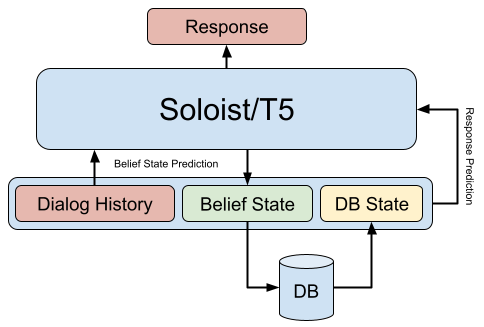
\includegraphics[width=0.8\textwidth]{figures/Soloist.png}
\caption{Soloist approach \cite{peng2020soloist}. Instead of using the GPT-2 Model \cite{radford2019language}, we use the T5 Model \cite{raffel2019exploring}.}
\label{fig:soloist}
\end{figure*}
Due to recent progress in sequence-to-sequence (seq2seq) models \cite{radford2019language, raffel2019exploring} recent work tries to fuse the NLU, dialogue management and NLG units into one seq2seq model like in \cite{peng2020soloist}.  
\section{Theory}
In this section we introduce the different approaches. \textbf{TODO}
\subsection{Soloist}The \textit{Soloist}\cite{peng2020soloist} approach fuses the different units into two seq2seq steps that are executed sequentially as shown in \autoref{fig:soloist}. In the first step, the previous dialogue history is used to predict the next belief state. The belief state is then parsed and transformed into a suitable format for the given knowledge base. The response of the knowledge base is then concatenated with the dialogue history and the belief state. The concatenation is fed into the model again in order to predict the next system response.\\
The Authors introduced three different training tasks:
\begin{enumerate}
\item \textbf{Belief Prediction}\\
The belief state is predicted as a seq2seq task. Thereby, the loss is calculated by the cross entropy loss of the target belief state sequence and the predicted belief state sequence.  
\item \textbf{Ground Response Generation}\\
The response generation is again a seq2seq task and uses the same criterion than the previous task.
\item \textbf{Contrastive Objective}\\
Beside optimising the similarity of the predicted and the ground truth sequences it is an essential part of the agent to place the correct information in the respective slots in the belief state or response. The authors therefore suggests a task that tried to enhance the awareness of the model towards incorrect target sequences. For that we sample normal target sequences from our dataset and we sample corrupted target sequences where the key information (eg. theatre location, movie name) is replaced by a random key information from the dataset. Based on the samples we apply a binary classification given the output of the models encoder to predict if the sequence is corrupted or not. The loss is calculated by the binary cross entropy loss. 
\end{enumerate}
\subsection{Soloist Modifications}
\begin{figure*}[!h]
\centering
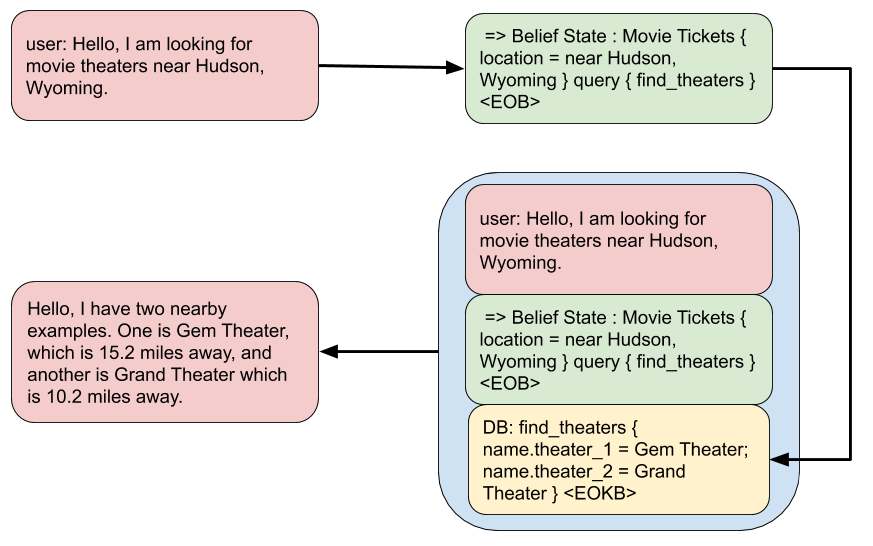
\includegraphics[width=0.8\textwidth]{figures/Soloist_Data.png}
\caption{An example in the format of \cite{peng2020soloist} with additional query word.}
\label{fig:soloistdata}
\end{figure*}
Due to resource limitations we decided to scale down the model described in \cite{peng2020soloist}. The authors implementation is based on the GPT-2 Model\cite{radford2019language} implemented by the Huggingface Transformers\cite{wolf2019huggingface}. In order to reduce the required resources we decided to take the T5-small\cite{raffel2019exploring} model. The GPT-2 Model has 117M parameters whereas T5-small has only 60M parameters\footnote{\url{https://huggingface.co/transformers/pretrained_models.html}} but still performs reasonably well.
Additionally, we modified the \textit{Belief State Prediction} task by adding an additional query word to the target sequence. The query word is used to properly transform the belief state to a format that can be used to query data from the knowledge base. An example of modified format is shown in \autoref{fig:soloistdata}. 

\section{Experimental Setup}
In this section we describe the different training setups. \textbf{TODO} 
\subsection{Soloist Setup}
The dataset that is used in \cite{peng2020soloist} they use the MultiWOZ dataset \cite{budzianowski2020multiwoz}. The MultiWOZ dataset is a multi domain dialogue dataset. Due to resource limitations and due to the smaller model that is used in this work we decided to only select one domain for training and validation. The selected domain from the MultiWOZ dataset is the \textit{Movie Ticket} domain, where the system has to guide the used through the ordering process. 

The model was trained with free available resources provided by Google Colab\footnote{\url{https://colab.research.google.com/}}.
\section{Results}


\section{Conclusions}


\section*{Acknowledgements}


\bibliographystyle{IEEEtran}
\bibliography{literature}

\end{document}
